\begin{figure}[tbp]
\begin{center}
\includegraphics[width=0.48\textwidth]{figure/cl_correlation_z1_z2.eps}
\end{center}
\vspace{-0.7cm}
\caption{The correlation coefficient r between real kSZ $P_{\Theta_{kSZ}}$ 
and reconstructed kSZ $P_{\hat \Theta_{kSZ}}$.
}
\label{fig:r}
\end{figure}
\label{ssec:tide}

To test the algorithm, six $N$-body simulations are performed with the
$\mr{CUBEP}^3\mr{M}$ code \cite{2013:code}, each evolving $1024^3$ particles in a $(1.2\mr{Gpc}/h)^3$ box. 
Simulation parameters are set as: Hubble parameter $h=0.678$, baryon
density $\Omega_{b}=0.049$, dark matter density $\Omega_{c}=0.259$,
amplitude of primordial curvature power spectrum $A_s=2.139\times10^{-9}$ at 
$k_0=0.05\;\mr{Mpc}^{-1}$ and scalar spectral index $n_s=0.968$.

Simulated density and velocity fields at $z=1,2$ are output 
and used to generate kSZ signal. 


To avoid manipulating noises, 
we perform tidal reconstruction on most conservative estimates, i.e. 
$R_\parallel=15$ Mpc/h, $k_\mr{max}=0.6$ h/Mpc, $\ell_\mr{max}=100$ for $z=1$; 
and $R_\parallel=10$ Mpc/h, $k_\mr{max}=0.4$ h/Mpc, $\ell_\mr{max}=100$ for $z=2$. 

The cross correlation between $\hat v_z^\mr{tide}$ and $v_z$ are demonstrated in Fig.\ref{fig:v}. 
Important modes for velocity fields (within redline of Fig.\ref{fig:k3v} lower label) are well extracted with correlations greater than $0.7$. 
%The reconstruction on $z=2$ is slightly worse than $z=1$ 
%due to stronger foreground and lower resolution. 

Combining reconstructed velocity field with density fields of different conditions, we get 21cm-reconstructed kSZ signals. 
Their correlation coefficients with exact kSZ are 
demonstrated in Fig.\ref{fig:r}. 
Even with identical tidal reconstructed velocity field, 
better foreground techneque can improve the correlation coefficient by 0.2. 
If the foreground is removed clean enough for more modes to be 
used in tidal reconstruction procedure, 
the improvement will be more notable.
Resolution of facility will improve the reconstruction on higher $\ell$, 
consisting with previous analysis.



